%% LyX 1.3 created this file.  For more info, see http://www.lyx.org/.
%% Do not edit unless you really know what you are doing.
\documentclass[english, 12pt]{article}
\usepackage{times}
%\usepackage{algorithm2e}
\usepackage{url}
\usepackage{bbm}
\usepackage[T1]{fontenc}
\usepackage[latin1]{inputenc}
\usepackage{geometry}
\geometry{verbose,letterpaper,tmargin=2cm,bmargin=2cm,lmargin=1.5cm,rmargin=1.5cm}
\usepackage{rotating}
\usepackage{color}
\usepackage{graphicx}
\usepackage{subcaption}
\usepackage{amsmath, amsthm, amssymb}
\usepackage{setspace}
\usepackage{lineno}
\usepackage{hyperref}
\usepackage{bbm}
\usepackage{makecell}

%\renewcommand{\arraystretch}{1.8}

%\usepackage{xr}
%\externaldocument{SCT-supp}

%\linenumbers
%\doublespacing
\onehalfspacing
%\usepackage[authoryear]{natbib}
\usepackage{natbib} \bibpunct{(}{)}{;}{author-year}{}{,}

%Pour les rajouts
\usepackage{color}
\definecolor{trustcolor}{rgb}{0,0,1}

\usepackage{dsfont}
\usepackage[warn]{textcomp}
\usepackage{adjustbox}
\usepackage{multirow}
\usepackage{graphicx}
\graphicspath{{figures/}}
\DeclareMathOperator*{\argmin}{\arg\!\min}

\let\tabbeg\tabular
\let\tabend\endtabular
\renewenvironment{tabular}{\begin{adjustbox}{max width=0.9\textwidth}\tabbeg}{\tabend\end{adjustbox}}

\makeatletter

%%%%%%%%%%%%%%%%%%%%%%%%%%%%%% LyX specific LaTeX commands.
%% Bold symbol macro for standard LaTeX users
%\newcommand{\boldsymbol}[1]{\mbox{\boldmath $#1$}}

%% Because html converters don't know tabularnewline
\providecommand{\tabularnewline}{\\}

\usepackage{babel}
\makeatother


\begin{document}


\title{Performing highly efficient genome scans for local adaptation with R package pcadapt version 4}
\author{Florian Priv\'e,$^{\text{1,2,}*}$ Keurcien Luu,$^{\text{2}}$ Bjarni J. Vilhj\'almsson$^{\text{1}}$ and Michael G.B. Blum$^{\text{2,3}}$}

\date{~ }
\maketitle

\noindent$^{\text{\sf 1}}$National Centre for Register-based Research, Aarhus University, Aarhus, 8210, Denmark. \\
\noindent$^{\text{\sf 2}}$Laboratoire TIMC-IMAG, UMR 5525, Univ.\ Grenoble Alpes, La Tronche, 38700, France. \\
\noindent$^{\text{\sf 3}}$OWKIN France, Paris, 75010, France. \\
\noindent$^\ast$To whom correspondence should be addressed.\\

\noindent Contacts:
\begin{itemize}
\item \url{florian.prive.21@gmail.com}
\end{itemize}

\vspace*{5em}

\abstract{
R package pcadapt is a user-friendly R package for performing genome scans for local adaptation. 
Here we present version 4 of pcadapt which substantially improves computational efficiency while providing similar results. 
This improvement is made possible by using a different format for storing genotypes and a different algorithm for computing principal components of the genotype matrix, which is the most computationally demanding step in method pcadapt.
These changes are seamlessly integrated into the existing pcadapt package, and users will experience a large reduction in computation time (by a factor of 20 to 60 in our analyses) as compared to previous versions.
}


%%%%%%%%%%%%%%%%%%%%%%%%%%%%%%%%%%%%%%%%%%%%%%%%%%%%%%%%%%%%%%%%%%%%%%%%%%%%%%%%

\clearpage

We developed the R package pcadapt as a method to detect signs of local adaptation in genetic data \cite[]{luu2017pcadapt}.
There are two main functions in the package: \texttt{read.pcadapt} which makes sure the data is in the right format and \texttt{pcadapt} which performs computations.
The pcadapt method first computes the Principal Component Analysis (PCA) of a scaled genotype matrix.
It then regresses all variants onto the resulting PCs to get a matrix of Z-scores (i.e.\ one Z-score for each variant and each PC).
Then, it computes robust Mahalanobis distances of these Z-scores to integrate all PCA dimensions in one multivariate distance for each variant \cite[]{luu2017pcadapt}.
These distances approximately follow a Chi-squared distribution, which enables derivation of one p-value for each genetic variant.
In essence, the pcadapt method tests how much each variant is associated with population structure, assuming that outlier variants are indicative of local adaptation.


%%%%%%%%%%%%%%%%%%%%%%%%%%%%%%%%%%%%%%%%%%%%%%%%%%%%%%%%%%%%%%%%%%%%%%%%%%%%%%%%

Previous versions of package pcadapt used format `pcadapt', which is a text file of characters separated by spaces where each line stores all samples' genotypes for one variant (0, 1, 2, and 9 for missing values).
It was also possible to convert from `ped' and `vcf' files to format `pcadapt'.
In pcadapt v4, the preferred format is now the PLINK `bed' format \cite[]{purcell2007plink}. 
Format `bed' is very compact; it stores each genotype using only 2 bits, making it 8 times smaller than the corresponding `pcadapt' file.
Moreover, format `bed' can be memory-mapped to be used in both R and C++ almost as a standard R(cpp) matrix; see e.g.\ R package BEDMatrix that provides matrix-like accessors to `bed' files \cite[]{grueneberg2019bgdata}.
Format `bed' is also advantageous because the widely-used software PLINK can be used to convert `ped' and `vcf' files to `bed' files, and to perform quality control \cite[]{chang2015second}.
For an existing `pcadapt' file, function \texttt{read.pcadapt} now creates a new file with extension `.pcadapt.bed' to be used by the main function \texttt{pcadapt}. 
Updating to version 4 is seamless for the user.

Previous versions of pcadapt computed the eigen decomposition of the Genetic Relationship Matrix (GRM).
In pcadapt v4, we use the implicitly restarted Arnoldi method (IRAM), which is both fast and accurate for computing first PCs \cite[]{Lehoucq1996,abraham2017flashpca2,prive2017efficient}.
To compare the performance of the newest version of R package pcadapt (v4.1.0 here) with previously published versions (v3.0.4 here), we use publicly available data on 4342 domestic dogs genotyped at 144,474 variants after quality control \cite[]{hayward2016complex}. 
Function \texttt{pcadapt} v3.0.4 takes 2111 seconds (35 minutes) to complete for this data. The bulk of this time is spent computing the GRM ($O(N^2 P)$, where $N$ is the number of samples and $P$ the number of variants).
With pcadapt v4.1.0, it takes only 35, 60 and 102 seconds to run for K=5, 10 and 20 PCs respectively (Figure \ref{fig:timings}, $\sim\!O(N P K)$).
This represents a 60, 35 and 20 folds improvement in computation time.


%%%%%%%%%%%%%%%%%%%%%%%%%%%%%%%%%%%%%%%%%%%%%%%%%%%%%%%%%%%%%%%%%%%%%%%%%%%%%%%%

Linkage disequilibrium (LD) can confound genome scans in admixed populations \cite[]{price2008long,abdellaoui2013population,galinsky2016fast}.
In previous versions of pcadapt, the only way to deal with this problem was to reduce K, the number of principal components (PCs) used by pcadapt, to include PCs capturing population structure only.
In version 4, we have added an option for performing LD clumping that removes variants in LD.
This ensures that more PCs capture population structure instead of LD structure \cite[]{prive2017efficient}.


%%%%%%%%%%%%%%%%%%%%%%%%%%%%%%%%%%%%%%%%%%%%%%%%%%%%%%%%%%%%%%%%%%%%%%%%%%%%%%%%

Overall, version 4 of R package pcadapt is much more efficient in terms of disk space, memory and time requirements compared to its previous versions.
This enables the analysis of large genotype datasets using a personal laptop.
Moreover, using the PLINK `bed' format instead of format `pcadapt' makes pcadapt easier to use along with PLINK, which can be used for file conversion and quality control.
Therefore pcadapt v4 supports all formats that can be converted to the `bed' format, such as `vcf' and `ped'. 
As for existing `pcadapt' files, they are seamlessly converted to format `bed' when using function \texttt{read.pcadapt}, which makes the new version backward compatible.
Most users analysing small datasets will likely not even notice the changes in version 4.
Moreover, results are expected to be very similar (see Supplementary Note).
However, as sample sizes continue to grow, the importance of computational efficiency and robust methods also grows, and this is exactly what we address in version 4 of pcadapt.


\begin{figure}[!htpb]
	\centerline{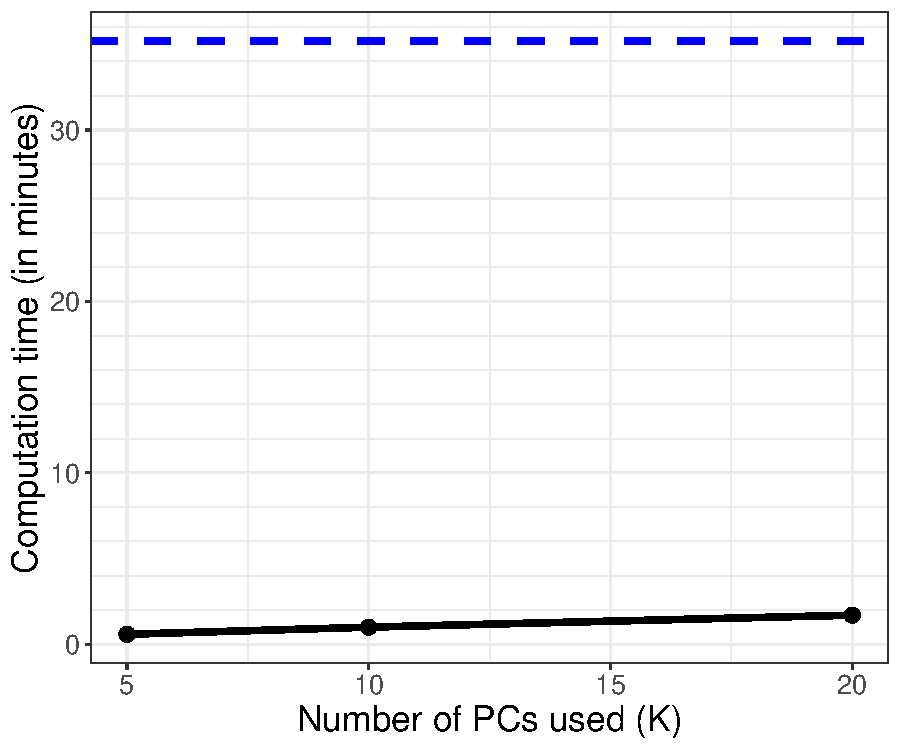
\includegraphics[width=0.7\textwidth]{timings.pdf}}
	\caption{Computation times of \texttt{pcadapt} as a function of the number of PCs used. Black points represent timings with pcadapt v4, and the dashed blue line represents the timing with v3, which is independent of the number of PC used. \label{fig:timings}}
\end{figure}

%%%%%%%%%%%%%%%%%%%%%%%%%%%%%%%%%%%%%%%%%%%%%%%%%%%%%%%%%%%%%%%%%%%%%%%%%%%%%%%%

\clearpage

\section*{Software and code availability}

R package pcadapt is available on CRAN. 
It also has a GitHub repository where you can open issues (\url{https://github.com/bcm-uga/pcadapt/issues}).
A tutorial on using pcadapt to detect local adaptation is available at \url{https://bcm-uga.github.io/pcadapt/articles/pcadapt.html}.
The code used in this paper is available at \url{https://github.com/bcm-uga/pcadapt/tree/master/new-paper/code}.

\section*{Acknowledgements}

F.P.\ and B.V.\ are supported by the Danish National Research Foundation (Niels Bohr Professorship to John McGrath).
The authors thank Katherine Musliner for her feedback on text.

\section*{Declaration of Interests}

Michael Blum is now an employee of OWKIN France.
The other authors declare no competing interests.

%%%%%%%%%%%%%%%%%%%%%%%%%%%%%%%%%%%%%%%%%%%%%%%%%%%%%%%%%%%%%%%%%%%%%%%%%%%%%%%%

\clearpage

\bibliographystyle{natbib}
\bibliography{refs}

%%%%%%%%%%%%%%%%%%%%%%%%%%%%%%%%%%%%%%%%%%%%%%%%%%%%%%%%%%%%%%%%%%%%%%%%%%%%%%%%

\clearpage
%\section*{Supplementary Materials}
%
%\renewcommand{\thefigure}{S\arabic{figure}}
%\setcounter{figure}{0}
%\renewcommand{\thetable}{S\arabic{table}}
%\setcounter{table}{0}


%%%%%%%%%%%%%%%%%%%%%%%%%%%%%%%%%%%%%%%%%%%%%%%%%%%%%%%%%%%%%%%%%%%%%%%%%%%%%%%%

\clearpage

%%%%%%%%%%%%%%%%%%%%%%%%%%%%%%%%%%%%%%%%%%%%%%%%%%%%%%%%%%%%%%%%%%%%%%%%%%%%%%%%

\end{document}
